% -----------------------------------------------
% Modelo UFT para Trabalhos Acadêmicos
% Adaptado e mantido por Wenes (Libertário)
% Baseado no projeto abnTeX2, porém modificado para atender às diretrizes
% visuais e estruturais da Universidade Federal do Tocantins (UFT).
% Esta versão não é oficial e não substitui os modelos originais do abnTeX2.
% -----------------------------------------------
\documentclass[
	12pt,				% Tamanho da fonte
    oneside,            % Garante margens iguais (não alternadas)
	a4paper,			% tamanho do papel. 
	english,			% idioma adicional para hifenização
	french,				% idioma adicional para hifenização
	spanish,			% idioma adicional para hifenização
	brazilian,		    % o último idioma é o principal do documento
	]{abntex2}
% -----------------------------------------------



% -----------------------------------------------
% -------------Pacotes fundamentais-------------- 
% -----------------------------------------------
\usepackage{lmodern}			% Usa a fonte Latin Modern
\usepackage[T1]{fontenc}		% Selecao de codigos de fonte.
\usepackage[utf8]{inputenc}		% Codificacao do documento (conversão automática dos acentos)
\usepackage{indentfirst}		% Indenta o primeiro parágrafo de cada seção.
\usepackage{color}				% Controle das cores
\usepackage{graphicx}			% Inclusão de gráficos
\usepackage{microtype} 			% para melhorias de justificação
% -----------------------------------------------


% -----------------------------------------------
\usepackage{lipsum}	% para geração de texto------
% -----------------------------------------------


% -----------------------------------------------
% -------------Pacotes de citações---------------
% -----------------------------------------------
\usepackage[backend=biber,style=abnt,language=brazil]{biblatex}
\addbibresource{Referencias.bib}
\usepackage{csquotes}             % Recomendado pelo biblatex 
\usepackage{etoolbox}             % Auxilia na justificação da bibliografia
\AtBeginBibliography{\justifying} % Ativa a justificação da bibliografia
\usepackage{ragged2e}
% -----------------------------------------------



% -----------------------------------------------
% --------VISUALIZAÇÃO E ESTABILIDADE------------
% -----------------------------------------------
\usepackage{tikz}         % Gerar imagem de exemplo
\usepackage{pgfplots}     % Funções matemática
\pgfplotsset{compat=1.18} % Garante compatibilidade
\usepackage{subcaption}   % Permite criar subfaturas
\usepackage{float}        % Adiciona a opção de posicionamento
\usepackage{amssymb}      % Necessário para símbolos matemáticos
\usepackage{amsmath}      % Necessário para comandos como \text{}
% -----------------------------------------------



% -----------------------------------------------
% -Informações para Folha de Rosto e Contracapa--
% -----------------------------------------------
\titulo{Modelo UFT para\\ Projeto de Pesquisa em \abnTeX}
\autor{Editado por Wenes Aquino}
\local{Palmas}
\data{2025, v-1.0}

\instituicao{%
  Universidade Federal do Tocantins - UFT\\
  Campus Universitário de Palmas\\
  Curso de Licenciatura em Computação}
  
\tipotrabalho{Projeto de Pesquisa}

\preambulo{Projeto de pesquisa apresentado como 
    parte dos requisitos para avaliação na Universidade 
    Federal do Tocantins (UFT). Este modelo foi adaptado 
    e personalizado com ajustes visuais, estruturais 
    e técnicos, servindo também para testar o espaço 
    disponível e a formatação utilizada na contracapa 
    deste documento.}
% -----------------------------------------------


% -----------------------------------------------
\makeatletter
\hypersetup{
    colorlinks=false,  % Desativa links coloridos
    pdfborder={0 0 0}, % Remove o retângulo dos links
}
\makeatother
% -----------------------------------------------


% -----------------------------------------------
% ----Espaçamentos entre linhas e parágrafos----- 
% -----------------------------------------------
\setlength{\parindent}{1.3cm} % O tamanho do parágrafo é dado por:
\setlength{\parskip}{0.2cm}   % Espaçamento entre parágrafo
% -----------------------------------------------


% -----------------------------------------------
% ---------------Compila o índice----------------
% -----------------------------------------------
\makeindex
% -----------------------------------------------




% -----------------------------------------------
\begin{document} % Início do documento-----------
% -----------------------------------------------
\nocite{*} % Inclui todas referências na página
\selectlanguage{brazilian}
\frenchspacing % Retira espaço extra obsoleto entre as frases.
% -----------------------------------------------



% -----------------------------------------------
% ------------ELEMENTOS PRÉ-TEXTUAIS-------------
% -----------------------------------------------
% \pretextual


% -----------------------------------------------
% ----------FOLHA DE ROSTO E CONTRACAPA----------
% -----------------------------------------------
\imprimircapa % Está é Folha de Rosto
% -----------------------------------------------
\imprimirfolhaderosto % Esta é Contracapa
% -----------------------------------------------



% -----------------------------------------------
% -----------------ILUSTRAÇÕES-------------------
% -----------------------------------------------
\pdfbookmark[0]{\listfigurename}{lof}
\listoffigures*
\cleardoublepage
% -----------------------------------------------



% -----------------------------------------------
% ------------------TABELAS----------------------
% -----------------------------------------------
\pdfbookmark[0]{\listtablename}{lot}
\listoftables*
\cleardoublepage
% -----------------------------------------------



% -----------------------------------------------
% ------------ABREVIATURAS E SIGLAS--------------
% -----------------------------------------------
\begin{siglas}
    % Siglas Originais
    \item[ABNT] Associação Brasileira de Normas Técnicas
    \item[abnTeX] ABsurdas Normas para TeX
    \item[ABNTC] Analistas de Burrocracia e Normas Tecnicamente Complicadas
    \item[ABNTT] Associação Brasileira de Normas Totalmente Travadas
    \item[ABNTE] Agrupamento Brasileiro de Normas Terrivelmente Escritas
    \item[ABNTX] Ajustes Básicos de Nomenclatura para Trabalhos Extraordinários
    
    % Siglas de Computação/TI
    \item[UML] Unified Modeling Language (Linguagem de Modelagem Unificada)
    \item[VBA] Visual Basic for Applications (Conhecimento em automação de planilhas)
    \item[BIOS] Basic Input/Output System (Sistema Básico de Entrada/Saída)
    
    % Siglas de Energia Solar (Sistemas Fotovoltaicos)
    \item[UFV] Usina Fotovoltaica
    \item[MPPT] Maximum Power Point Tracking (Rastreamento do Ponto de Máxima Potência)
    \item[PVS] Photovoltaic System (Sistema Fotovoltaico)
    
    % Siglas da Instituição
    \item[UFT] Universidade Federal do Tocantins
    \item[UAB] Universidade Aberta do Brasil
\end{siglas}
% -----------------------------------------------



% -----------------------------------------------
% ------------------ SÍMBOLOS -------------------
% -----------------------------------------------
\begin{simbolos}
    % --- Matemática/Computação ---
    \item[$ \mathbb{N} $] Conjunto dos números naturais (Nomenclatura Padrão).
    \item[$ \Sigma $] Símbolo de Somatório ou Sigma (Usado em Análise de Dados).
    \item[$ \land $] Operador Lógico AND (Conjunção).
    \item[$ \lor $] Operador Lógico OR (Disjunção).
    \item[$ \nabla $] Operador Nabla (Usado em Cálculo Vetorial).
    
    % --- Eletrônica/Sistemas Fotovoltaicos ---
    \item[$ \Omega $] Ohm (Unidade de resistência elétrica).
    \item[$ \text{V} $] Volt (Unidade de Tensão Elétrica, $V=R \cdot I$).
    \item[$ I_L $] Corrente de Carga (Load Current) em Sistemas Fotovoltaicos.
    \item[$ \text{P}_{\text{MPP}} $] Ponto de Máxima Potência (Maximum Power Point).
    
    % --- LaTeX/Documentação (Sua Expertise) ---
    \item[$ \texttt{\symbol{92}} $] Símbolo de Barra Invertida (Backslash) (Comando fundamental do \LaTeX).
\end{simbolos}
% -----------------------------------------------



% -----------------------------------------------
% ------------------SUMÁRIO----------------------
% -----------------------------------------------
\pdfbookmark[0]{\contentsname}{toc}
\tableofcontents*
\cleardoublepage
% -----------------------------------------------



% -----------------------------------------------
% --------------ELEMENTOS TEXTUAIS---------------
% -----------------------------------------------
\textual



% -----------------------------------------------
% -----------------Introdução--------------------
% -----------------------------------------------
\chapter*[Introdução]{Introdução}
\addcontentsline{toc}{chapter}{Introdução}

\lipsum[1-2] % Gera texto de exemplo para preencher a página.
\lipsum[2] \footnote{\url{http://www.latex-project.org/lppl.txt}}.
% -----------------------------------------------



% -----------------------------------------------
% -------------Capitulo de Textual---------------  
% -----------------------------------------------
\chapter{Funções Matemáticas}

\section{Morbi orci nisl hendrerit}
\lipsum[1-2] % Gera texto de exemplo para preencher a página. 
\cite{talbot2012}


\newpage % Nova Página 
% -----------------------------------------------
\section{Exemplo de Gráficos de Funções Matemáticas}

\noindent Esta seção demonstra o poder do LaTeX para gerar gráficos vetoriais de alta qualidade, que populam automaticamente a Lista de Ilustrações.

% -----------------------------------------------
% --------------1. FUNÇÃO LINEAR----------------- 
% -----------------------------------------------
\begin{figure}[H]
    \centering
    \begin{tikzpicture}
    \begin{axis}[
        title={Função Linear $f(x)=x$},
        axis lines=middle,
        xlabel={$x$},
        ylabel={$f(x)$},
        xmin=-2, xmax=2, ymin=-2, ymax=2]
    \addplot[blue, thick] {x};
    \end{axis}
    \end{tikzpicture}
    \caption{Gráfico de uma função linear $f(x)=x$.}
    \label{fig:funcao_linear}
\end{figure}

% -----------------------------------------------
% ------------2. FUNÇÃO QUADRÁTICA---------------
% -----------------------------------------------
\begin{figure}[H]
    \centering
    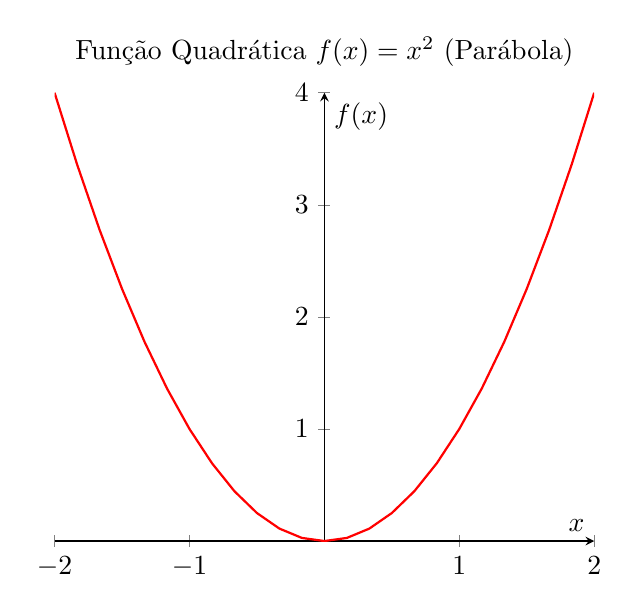
\begin{tikzpicture}
    \begin{axis}[
        title={Função Quadrática $f(x)=x^2$ (Parábola)},
        axis lines=middle,
        xlabel={$x$},
        ylabel={$f(x)$},
        xmin=-2, xmax=2, ymin=0, ymax=4]
    \addplot[red, thick, domain=-2:2] {x^2};
    \end{axis}
    \end{tikzpicture}
    \caption{Gráfico de uma função quadrática $f(x)=x^2$, representando uma parábola.}
    \label{fig:funcao_quadratica}
\end{figure}

% -----------------------------------------------
% --------------3. FUNÇÃO SENOIDE--------------- 
% -----------------------------------------------
\begin{figure}[H]
    \centering
    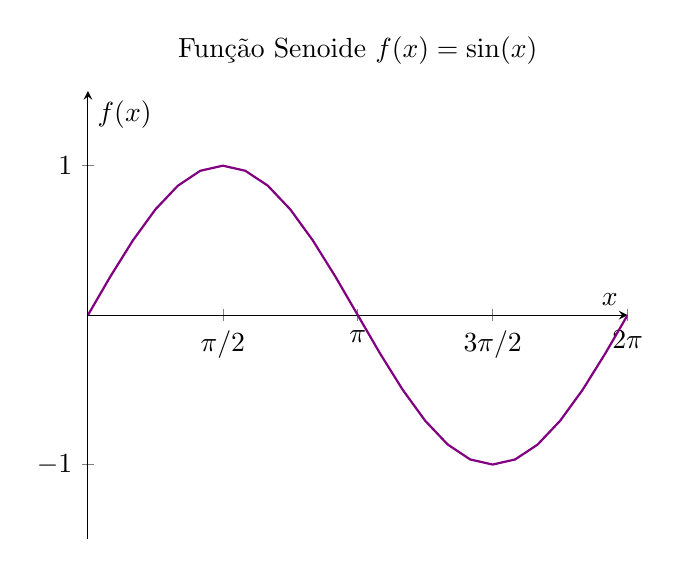
\begin{tikzpicture}
    \begin{axis}[
        title={Função Senoide $f(x)=\sin(x)$},
        axis lines=middle,
        xlabel={$x$},
        ylabel={$f(x)$},
        xmin=0, xmax=360, ymin=-1.5, ymax=1.5,
        xtick={0, 90, 180, 270, 360},
        xticklabels={0, $\pi/2$, $\pi$, $3\pi/2$, $2\pi$}
    ]
    \addplot[violet, thick, domain=0:360] ({x}, {sin(x)});
    \end{axis}
    \end{tikzpicture}
    \caption{Gráfico da função senoide $f(x)=\sin(x)$, demonstrando periodicidade.}
    \label{fig:funcao_senoide}
\end{figure}

% -----------------------------------------------
% ------------4. FUNÇÃO EXPONENCIAL-------------- 
% -----------------------------------------------
\begin{figure}[H]
    \centering
    \begin{tikzpicture}
    \begin{axis}[
        title={Função Exponencial $f(x)=e^x$},
        axis lines=middle,
        xlabel={$x$},
        ylabel={$f(x)$},
        xmin=-2, xmax=2, ymin=0, ymax=8,
        domain=-2:2]
    \addplot[green!60!black, thick] {exp(x)};
    \end{axis}
    \end{tikzpicture}
    \caption{Gráfico de uma função exponencial $f(x)=e^x$, representando crescimento acentuado.}
    \label{fig:funcao_exponencial}
\end{figure}

% -----------------------------------------------
% -----------5. FUNÇÃO LOGARÍTMICA--------------- 
% -----------------------------------------------
\begin{figure}[H]
    \centering
    \begin{tikzpicture}
    \begin{axis}[
        title={Função Logarítmica $f(x)=\ln(x)$},
        axis lines=middle,
        xlabel={$x$},
        ylabel={$f(x)$},
        xmin=0, xmax=5, ymin=-2, ymax=2,
        domain=0.01:5]
    \addplot[orange, thick] {ln(x)};
    \end{axis}
    \end{tikzpicture}
    \caption{Gráfico da função logarítmica natural $f(x)=\ln(x)$, mostrando o crescimento lento.}
    \label{fig:funcao_logaritmica}
\end{figure}
% -----------------------------------------------




\newpage % Nova Página 
% -----------------------------------------------
\section{Exemplo de Lista de Tabelas}
% -----------------------------------------------

\noindent Esta seção demonstra a correta formatação ABNT para tabelas e garante o preenchimento da Lista de Tabelas.

% -----------------------------------------------
\begin{table}[H]
    \centering
    \caption{Resultados dos Testes de Velocidade (Baseline)}
    \label{tab:velocidade_baseline}
    \begin{tabular}{lcc}
        \toprule
        Módulo & Tempo (ms) & Status \\
        \midrule
        Login & 120 & OK \\
        Busca & 450 & Crítico \\
        \bottomrule
    \end{tabular}
\end{table}

\begin{table}[H]
    \centering
    \caption{Recursos Utilizados por Componente}
    \label{tab:recursos_comp}
    \begin{tabular}{lrr}
        \toprule
        Componente & RAM (MB) & CPU (\%) \\
        \midrule
        Backend API & 512 & 30 \\
        Frontend UI & 128 & 15 \\
        \bottomrule
    \end{tabular}
\end{table}

\begin{table}[H]
    \centering
    \caption{Cronograma de Implementação (Fase Alpha)}
    \label{tab:cronograma_alpha}
    \begin{tabular}{llr}
        \toprule
        Tarefa & Responsável & Prazo (Dias) \\
        \midrule
        Setup Inicial & Equipe T.I. & 5 \\
        Desenvolvimento & Programador & 15 \\
        \bottomrule
    \end{tabular}
\end{table}

\begin{table}[H]
    \centering
    \caption{Classificação de Bugs por Prioridade}
    \label{tab:bugs_prioridade}
    \begin{tabular}{lc}
        \toprule
        Prioridade & Incidência \\
        \midrule
        Crítica & 3 \\
        Média & 8 \\
        Baixa & 12 \\
        \bottomrule
    \end{tabular}
\end{table}

\begin{table}[H]
    \centering
    \caption{Comparativo de Linguagens de Programação}
    \label{tab:linguagens_comp}
    \begin{tabular}{ccc}
        \toprule
        Linguagem & Desempenho & Curva de Aprendizado \\
        \midrule
        Python & Médio & Baixa \\
        C++ & Alta & Alta \\
        \bottomrule
    \end{tabular}
\end{table}

\begin{table}[H]
    \centering
    \caption{Especificações do Painel Fotovoltaico}
    \label{tab:painel_foto}
    \begin{tabular}{lc}
        \toprule
        Parâmetro & Valor \\
        \midrule
        Potência Máx. & 350 W \\
        Eficiência & 20.5\% \\
        \bottomrule
    \end{tabular}
\end{table}
% -----------------------------------------------



\chapter{Suspendisse vel felis}

\section{Praesent enim elit}
\lipsum[6-7] % Gera texto de exemplo para preencher a página. 


\section{Curabitur et nunc}
\lipsum[8-10] % Gera texto de exemplo para preencher a página. 



\chapter{Cras non urna. Morbi eros pede}

\section{Nullam at lectus}
\lipsum[10-11] % Gera texto de exemplo para preencher a página. 

\section{Praesent pretium}
\lipsum[12-13] % Gera texto de exemplo para preencher a página. 




% -----------------------------------------------
% Finaliza a parte no bookmark do PDF
% para que se inicie o bookmark na raiz
% e adiciona espaço de parte no Sumário
% -----------------------------------------------
\phantompart




% -----------------------------------------------
% ----------------Conclusão----------------------
% -----------------------------------------------
\chapter*[Considerações Finais]{Considerações Finais}
\addcontentsline{toc}{chapter}{Considerações Finais}
\lipsum[31-33] % Gera texto de exemplo para preencher a página.



% -----------------------------------------------
% -----------ELEMENTOS PÓS-TEXTUAIS--------------
% -----------------------------------------------
\postextual



% -----------------------------------------------
% ----------Referências bibliográficas-----------
% -----------------------------------------------
\chapter*{Referências}                                               % Insere o título
\markboth{Referências}{Referências}                                  % Título "Referências" no cabeçalho.
\addtocontents{toc}{\protect\vspace{\baselineskip}}                  % Adiciona uma linha.
\addcontentsline{toc}{chapter}{\protect\MakeUppercase{REFERÊNCIAS}}  % Nível 'chapter' para linha grossos.
\printbibliography[heading=none]                                     % Imprime a bibliografia.
% -----------------------------------------------



% -----------------------------------------------
% -----------------APÊNDICE---------------------- 
% -----------------------------------------------
\begin{apendicesenv}
\partapendices % Imprime uma página indicando o início dos apêndices

\chapter{Quisque libero justo}

\section{Aliquam viverra arcu}
\lipsum[8-9] % Gera texto de exemplo para preencher a página. 

\section{Mauris consequat}
\lipsum[24-25] % Gera texto de exemplo para preencher a página. 

% -----------------------------------------------

\chapter{Nullam elementum}

\section{Quisque facilisis auctor sapien}
\lipsum[80-81] % Gera texto de exemplo para preencher a página. 

\section{Aliquam quis quam non metus}
\lipsum[34-35] % Gera texto de exemplo para preencher a página. 

\end{apendicesenv}
% -----------------------------------------------



% -----------------------------------------------
% ------------------ANEXOS-----------------------
% -----------------------------------------------
\begin{anexosenv}
\partanexos % Imprime uma página indicando o início dos anexos

\chapter{Morbi ultrices rutrum lorem}

\section{Pellentesque sodales}
\lipsum[40-41] % Gera texto de exemplo para preencher a página. 

\section{Curabitur diam tortor}
\lipsum[54-55] % Gera texto de exemplo para preencher a página. 

\section{Nullam elit sapien}
\lipsum[56-57] % Gera texto de exemplo para preencher a página. 

\end{anexosenv}
% -----------------------------------------------


\end{document} 